\documentclass[1p]{elsarticle_modified}
%\bibliographystyle{elsarticle-num}

%\usepackage[colorlinks]{hyperref}
%\usepackage{abbrmath_seonhwa} %\Abb, \Ascr, \Acal ,\Abf, \Afrak
\usepackage{amsfonts}
\usepackage{amssymb}
\usepackage{amsmath}
\usepackage{amsthm}
\usepackage{scalefnt}
\usepackage{amsbsy}
\usepackage{kotex}
\usepackage{caption}
\usepackage{subfig}
\usepackage{color}
\usepackage{graphicx}
\usepackage{xcolor} %% white, black, red, green, blue, cyan, magenta, yellow
\usepackage{float}
\usepackage{setspace}
\usepackage{hyperref}

\usepackage{tikz}
\usetikzlibrary{arrows}

\usepackage{multirow}
\usepackage{array} % fixed length table
\usepackage{hhline}

%%%%%%%%%%%%%%%%%%%%%
\makeatletter
\renewcommand*\env@matrix[1][\arraystretch]{%
	\edef\arraystretch{#1}%
	\hskip -\arraycolsep
	\let\@ifnextchar\new@ifnextchar
	\array{*\c@MaxMatrixCols c}}
\makeatother %https://tex.stackexchange.com/questions/14071/how-can-i-increase-the-line-spacing-in-a-matrix
%%%%%%%%%%%%%%%

\usepackage[normalem]{ulem}

\newcommand{\msout}[1]{\ifmmode\text{\sout{\ensuremath{#1}}}\else\sout{#1}\fi}
%SOURCE: \msout is \stkout macro in https://tex.stackexchange.com/questions/20609/strikeout-in-math-mode

\newcommand{\cancel}[1]{
	\ifmmode
	{\color{red}\msout{#1}}
	\else
	{\color{red}\sout{#1}}
	\fi
}

\newcommand{\add}[1]{
	{\color{blue}\uwave{#1}}
}

\newcommand{\replace}[2]{
	\ifmmode
	{\color{red}\msout{#1}}{\color{blue}\uwave{#2}}
	\else
	{\color{red}\sout{#1}}{\color{blue}\uwave{#2}}
	\fi
}

\newcommand{\Sol}{\mathcal{S}} %segment
\newcommand{\D}{D} %diagram
\newcommand{\A}{\mathcal{A}} %arc


%%%%%%%%%%%%%%%%%%%%%%%%%%%%%5 test

\def\sl{\operatorname{\textup{SL}}(2,\Cbb)}
\def\psl{\operatorname{\textup{PSL}}(2,\Cbb)}
\def\quan{\mkern 1mu \triangleright \mkern 1mu}

\theoremstyle{definition}
\newtheorem{thm}{Theorem}[section]
\newtheorem{prop}[thm]{Proposition}
\newtheorem{lem}[thm]{Lemma}
\newtheorem{ques}[thm]{Question}
\newtheorem{cor}[thm]{Corollary}
\newtheorem{defn}[thm]{Definition}
\newtheorem{exam}[thm]{Example}
\newtheorem{rmk}[thm]{Remark}
\newtheorem{alg}[thm]{Algorithm}

\newcommand{\I}{\sqrt{-1}}
\begin{document}

%\begin{frontmatter}
%
%\title{Boundary parabolic representations of knots up to 8 crossings}
%
%%% Group authors per affiliation:
%\author{Yunhi Cho} 
%\address{Department of Mathematics, University of Seoul, Seoul, Korea}
%\ead{yhcho@uos.ac.kr}
%
%
%\author{Seonhwa Kim} %\fnref{s_kim}}
%\address{Center for Geometry and Physics, Institute for Basic Science, Pohang, 37673, Korea}
%\ead{ryeona17@ibs.re.kr}
%
%\author{Hyuk Kim}
%\address{Department of Mathematical Sciences, Seoul National University, Seoul 08826, Korea}
%\ead{hyukkim@snu.ac.kr}
%
%\author{Seokbeom Yoon}
%\address{Department of Mathematical Sciences, Seoul National University, Seoul, 08826,  Korea}
%\ead{sbyoon15@snu.ac.kr}
%
%\begin{abstract}
%We find all boundary parabolic representation of knots up to 8 crossings.
%
%\end{abstract}
%\begin{keyword}
%    \MSC[2010] 57M25 
%\end{keyword}
%
%\end{frontmatter}

%\linenumbers
%\tableofcontents
%
\newcommand\colored[1]{\textcolor{white}{\rule[-0.35ex]{0.8em}{1.4ex}}\kern-0.8em\color{red} #1}%
%\newcommand\colored[1]{\textcolor{white}{ #1}\kern-2.17ex	\textcolor{white}{ #1}\kern-1.81ex	\textcolor{white}{ #1}\kern-2.15ex\color{red}#1	}

{\Large $\underline{11a_{110}~(K11a_{110})}$}

\setlength{\tabcolsep}{10pt}
\renewcommand{\arraystretch}{1.6}
\vspace{1cm}\begin{tabular}{m{100pt}>{\centering\arraybackslash}m{274pt}}
\multirow{5}{120pt}{
	\centering
	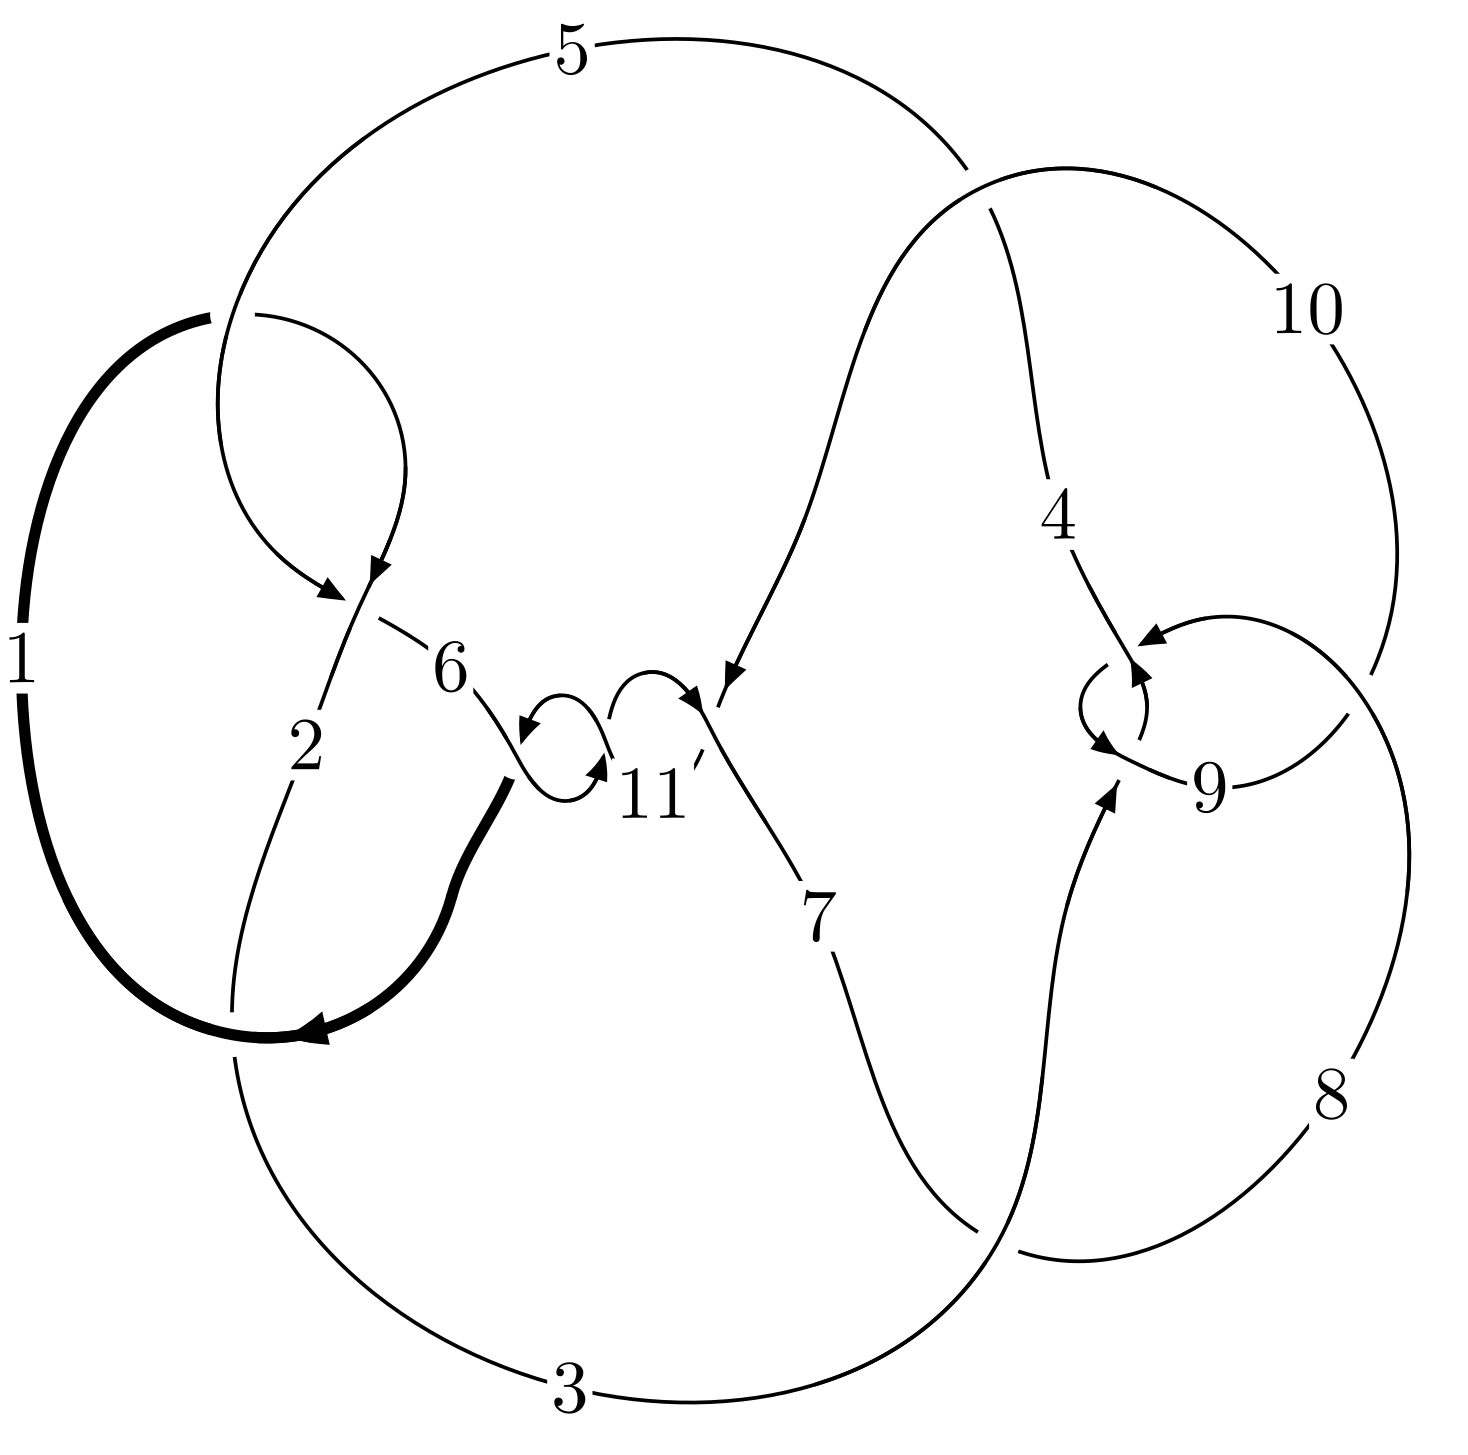
\includegraphics[width=112pt]{../../../GIT/diagram.site/Diagrams/png/359_11a_110.png}\\
\ \ \ A knot diagram\footnotemark}&
\allowdisplaybreaks
\textbf{Linearized knot diagam} \\
\cline{2-2}
 &
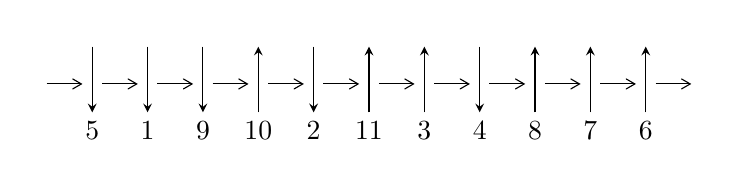
\begin{tikzpicture}[x=20pt, y=17pt]
	% nodes
	\node (C0) at (0, 0) {};
	\node (C1) at (1, 0) {};
	\node (C1U) at (1, +1) {};
	\node (C1D) at (1, -1) {5};

	\node (C2) at (2, 0) {};
	\node (C2U) at (2, +1) {};
	\node (C2D) at (2, -1) {1};

	\node (C3) at (3, 0) {};
	\node (C3U) at (3, +1) {};
	\node (C3D) at (3, -1) {9};

	\node (C4) at (4, 0) {};
	\node (C4U) at (4, +1) {};
	\node (C4D) at (4, -1) {10};

	\node (C5) at (5, 0) {};
	\node (C5U) at (5, +1) {};
	\node (C5D) at (5, -1) {2};

	\node (C6) at (6, 0) {};
	\node (C6U) at (6, +1) {};
	\node (C6D) at (6, -1) {11};

	\node (C7) at (7, 0) {};
	\node (C7U) at (7, +1) {};
	\node (C7D) at (7, -1) {3};

	\node (C8) at (8, 0) {};
	\node (C8U) at (8, +1) {};
	\node (C8D) at (8, -1) {4};

	\node (C9) at (9, 0) {};
	\node (C9U) at (9, +1) {};
	\node (C9D) at (9, -1) {8};

	\node (C10) at (10, 0) {};
	\node (C10U) at (10, +1) {};
	\node (C10D) at (10, -1) {7};

	\node (C11) at (11, 0) {};
	\node (C11U) at (11, +1) {};
	\node (C11D) at (11, -1) {6};
	\node (C12) at (12, 0) {};

	% arrows
	\draw[->,>={angle 60}]
	(C0) edge (C1) (C1) edge (C2) (C2) edge (C3) (C3) edge (C4) (C4) edge (C5) (C5) edge (C6) (C6) edge (C7) (C7) edge (C8) (C8) edge (C9) (C9) edge (C10) (C10) edge (C11) (C11) edge (C12) ;	\draw[->,>=stealth]
	(C1U) edge (C1D) (C2U) edge (C2D) (C3U) edge (C3D) (C4D) edge (C4U) (C5U) edge (C5D) (C6D) edge (C6U) (C7D) edge (C7U) (C8U) edge (C8D) (C9D) edge (C9U) (C10D) edge (C10U) (C11D) edge (C11U) ;
	\end{tikzpicture} \\
\hhline{~~} \\& 
\textbf{Solving Sequence} \\ \cline{2-2} 
 &
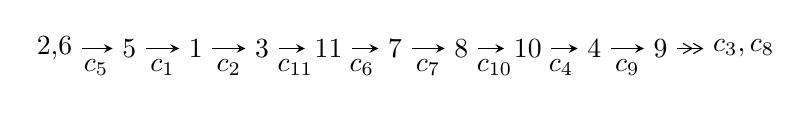
\begin{tikzpicture}[x=24pt, y=7pt]
	% node
	\node (A0) at (-1/8, 0) {2,6};
	\node (A1) at (1, 0) {5};
	\node (A2) at (2, 0) {1};
	\node (A3) at (3, 0) {3};
	\node (A4) at (4, 0) {11};
	\node (A5) at (5, 0) {7};
	\node (A6) at (6, 0) {8};
	\node (A7) at (7, 0) {10};
	\node (A8) at (8, 0) {4};
	\node (A9) at (9, 0) {9};
	\node (C1) at (1/2, -1) {$c_{5}$};
	\node (C2) at (3/2, -1) {$c_{1}$};
	\node (C3) at (5/2, -1) {$c_{2}$};
	\node (C4) at (7/2, -1) {$c_{11}$};
	\node (C5) at (9/2, -1) {$c_{6}$};
	\node (C6) at (11/2, -1) {$c_{7}$};
	\node (C7) at (13/2, -1) {$c_{10}$};
	\node (C8) at (15/2, -1) {$c_{4}$};
	\node (C9) at (17/2, -1) {$c_{9}$};
	\node (A10) at (41/4, 0) {$c_{3},c_{8}$};

	% edge
	\draw[->,>=stealth]	
	(A0) edge (A1) (A1) edge (A2) (A2) edge (A3) (A3) edge (A4) (A4) edge (A5) (A5) edge (A6) (A6) edge (A7) (A7) edge (A8) (A8) edge (A9) ;
	\draw[->>,>={angle 60}]	
	(A9) edge (A10);
\end{tikzpicture} \\ 

\end{tabular} \\

\footnotetext{
The image of knot diagram is generated by the software ``\textbf{Draw programme}" developed by Andrew Bartholomew(\url{http://www.layer8.co.uk/maths/draw/index.htm\#Running-draw}), where we modified some parts for our purpose(\url{https://github.com/CATsTAILs/LinksPainter}).
}\phantom \\ \newline 
\centering \textbf{Ideals for irreducible components\footnotemark of $X_{\text{par}}$} 
 
\begin{align*}
I^u_{1}&=\langle 
u^{48}- u^{47}+\cdots-4 u^3+1\rangle \\
\\
\end{align*}
\raggedright * 1 irreducible components of $\dim_{\mathbb{C}}=0$, with total 48 representations.\\
\footnotetext{All coefficients of polynomials are rational numbers. But the coefficients are sometimes approximated in decimal forms when there is not enough margin.}
\newpage
\renewcommand{\arraystretch}{1}
\centering \section*{I. $I^u_{1}= \langle u^{48}- u^{47}+\cdots-4 u^3+1 \rangle$}
\flushleft \textbf{(i) Arc colorings}\\
\begin{tabular}{m{7pt} m{180pt} m{7pt} m{180pt} }
\flushright $a_{2}=$&$\begin{pmatrix}0\\u\end{pmatrix}$ \\
\flushright $a_{6}=$&$\begin{pmatrix}1\\0\end{pmatrix}$ \\
\flushright $a_{5}=$&$\begin{pmatrix}1\\- u^2\end{pmatrix}$ \\
\flushright $a_{1}=$&$\begin{pmatrix}u\\- u^3+u\end{pmatrix}$ \\
\flushright $a_{3}=$&$\begin{pmatrix}- u^3\\u^5- u^3+u\end{pmatrix}$ \\
\flushright $a_{11}=$&$\begin{pmatrix}u^3\\- u^3+u\end{pmatrix}$ \\
\flushright $a_{7}=$&$\begin{pmatrix}u^6- u^4+1\\- u^6+2 u^4- u^2\end{pmatrix}$ \\
\flushright $a_{8}=$&$\begin{pmatrix}u^{14}-3 u^{12}+4 u^{10}- u^8+1\\- u^{16}+4 u^{14}-8 u^{12}+8 u^{10}-4 u^8-2 u^6+4 u^4-2 u^2\end{pmatrix}$ \\
\flushright $a_{10}=$&$\begin{pmatrix}u^9-2 u^7+u^5+2 u^3- u\\- u^9+3 u^7-3 u^5+u\end{pmatrix}$ \\
\flushright $a_{4}=$&$\begin{pmatrix}u^{20}-5 u^{18}+11 u^{16}-10 u^{14}-2 u^{12}+13 u^{10}-9 u^8+3 u^4- u^2+1\\- u^{20}+6 u^{18}-16 u^{16}+22 u^{14}-13 u^{12}-4 u^{10}+10 u^8-4 u^6- u^4\end{pmatrix}$ \\
\flushright $a_{9}=$&$\begin{pmatrix}- u^{39}+10 u^{37}+\cdots+4 u^3-2 u\\u^{41}-11 u^{39}+\cdots+2 u^3+u\end{pmatrix}$\\ \flushright $a_{9}=$&$\begin{pmatrix}- u^{39}+10 u^{37}+\cdots+4 u^3-2 u\\u^{41}-11 u^{39}+\cdots+2 u^3+u\end{pmatrix}$\\&\end{tabular}
\flushleft \textbf{(ii) Obstruction class $= -1$}\\~\\
\flushleft \textbf{(iii) Cusp Shapes $= 4 u^{47}-56 u^{45}+\cdots-8 u^2-2$}\\~\\
\newpage\renewcommand{\arraystretch}{1}
\flushleft \textbf{(iv) u-Polynomials at the component}\newline \\
\begin{tabular}{m{50pt}|m{274pt}}
Crossings & \hspace{64pt}u-Polynomials at each crossing \\
\hline $$\begin{aligned}c_{1},c_{5}\end{aligned}$$&$\begin{aligned}
&u^{48}+u^{47}+\cdots+4 u^3+1
\end{aligned}$\\
\hline $$\begin{aligned}c_{2}\end{aligned}$$&$\begin{aligned}
&u^{48}+27 u^{47}+\cdots+28 u^3+1
\end{aligned}$\\
\hline $$\begin{aligned}c_{3},c_{8}\end{aligned}$$&$\begin{aligned}
&u^{48}- u^{47}+\cdots-2 u^4+1
\end{aligned}$\\
\hline $$\begin{aligned}c_{4},c_{7}\end{aligned}$$&$\begin{aligned}
&u^{48}+u^{47}+\cdots-44 u+17
\end{aligned}$\\
\hline $$\begin{aligned}c_{6},c_{10},c_{11}\end{aligned}$$&$\begin{aligned}
&u^{48}+3 u^{47}+\cdots+8 u+1
\end{aligned}$\\
\hline $$\begin{aligned}c_{9}\end{aligned}$$&$\begin{aligned}
&u^{48}-25 u^{47}+\cdots-4 u^2+1
\end{aligned}$\\
\hline
\end{tabular}\\~\\
\newpage\renewcommand{\arraystretch}{1}
\flushleft \textbf{(v) Riley Polynomials at the component}\newline \\
\begin{tabular}{m{50pt}|m{274pt}}
Crossings & \hspace{64pt}Riley Polynomials at each crossing \\
\hline $$\begin{aligned}c_{1},c_{5}\end{aligned}$$&$\begin{aligned}
&y^{48}-27 y^{47}+\cdots-28 y^3+1
\end{aligned}$\\
\hline $$\begin{aligned}c_{2}\end{aligned}$$&$\begin{aligned}
&y^{48}-11 y^{47}+\cdots+308 y^2+1
\end{aligned}$\\
\hline $$\begin{aligned}c_{3},c_{8}\end{aligned}$$&$\begin{aligned}
&y^{48}+25 y^{47}+\cdots-4 y^2+1
\end{aligned}$\\
\hline $$\begin{aligned}c_{4},c_{7}\end{aligned}$$&$\begin{aligned}
&y^{48}-31 y^{47}+\cdots+2620 y+289
\end{aligned}$\\
\hline $$\begin{aligned}c_{6},c_{10},c_{11}\end{aligned}$$&$\begin{aligned}
&y^{48}+49 y^{47}+\cdots+56 y+1
\end{aligned}$\\
\hline $$\begin{aligned}c_{9}\end{aligned}$$&$\begin{aligned}
&y^{48}-3 y^{47}+\cdots-8 y+1
\end{aligned}$\\
\hline
\end{tabular}\\~\\
\newpage\flushleft \textbf{(vi) Complex Volumes and Cusp Shapes}
$$\begin{array}{c|c|c}  
\text{Solutions to }I^u_{1}& \I (\text{vol} + \sqrt{-1}CS) & \text{Cusp shape}\\
 \hline 
\begin{aligned}
u &= \phantom{-}0.958219 + 0.143307 I\end{aligned}
 & -1.66920 - 0.31218 I & -6.04929 + 0.55460 I \\ \hline\begin{aligned}
u &= \phantom{-}0.958219 - 0.143307 I\end{aligned}
 & -1.66920 + 0.31218 I & -6.04929 - 0.55460 I \\ \hline\begin{aligned}
u &= \phantom{-}0.914661 + 0.504015 I\end{aligned}
 & \phantom{-}4.41403 - 0.70127 I & \phantom{-}5.15173 + 2.65109 I \\ \hline\begin{aligned}
u &= \phantom{-}0.914661 - 0.504015 I\end{aligned}
 & \phantom{-}4.41403 + 0.70127 I & \phantom{-}5.15173 - 2.65109 I \\ \hline\begin{aligned}
u &= -1.046740 + 0.068635 I\end{aligned}
 & \phantom{-}0.77690 - 3.72476 I & -1.95300 + 3.66807 I \\ \hline\begin{aligned}
u &= -1.046740 - 0.068635 I\end{aligned}
 & \phantom{-}0.77690 + 3.72476 I & -1.95300 - 3.66807 I \\ \hline\begin{aligned}
u &= \phantom{-}1.011960 + 0.286206 I\end{aligned}
 & -2.55221 - 0.92643 I & -6.15695 + 0.73591 I \\ \hline\begin{aligned}
u &= \phantom{-}1.011960 - 0.286206 I\end{aligned}
 & -2.55221 + 0.92643 I & -6.15695 - 0.73591 I \\ \hline\begin{aligned}
u &= -0.950614 + 0.484261 I\end{aligned}
 & \phantom{-}0.72805 + 4.58119 I & \phantom{-}0.34102 - 6.39238 I \\ \hline\begin{aligned}
u &= -0.950614 - 0.484261 I\end{aligned}
 & \phantom{-}0.72805 - 4.58119 I & \phantom{-}0.34102 + 6.39238 I \\ \hline\begin{aligned}
u &= -1.021410 + 0.380117 I\end{aligned}
 & -1.89118 + 4.83513 I & -2.88338 - 8.66489 I \\ \hline\begin{aligned}
u &= -1.021410 - 0.380117 I\end{aligned}
 & -1.89118 - 4.83513 I & -2.88338 + 8.66489 I \\ \hline\begin{aligned}
u &= \phantom{-}0.963622 + 0.510991 I\end{aligned}
 & \phantom{-}3.78897 - 9.13187 I & \phantom{-}3.52711 + 9.35882 I \\ \hline\begin{aligned}
u &= \phantom{-}0.963622 - 0.510991 I\end{aligned}
 & \phantom{-}3.78897 + 9.13187 I & \phantom{-}3.52711 - 9.35882 I \\ \hline\begin{aligned}
u &= \phantom{-}0.080810 + 0.850812 I\end{aligned}
 & -0.65137 + 8.58815 I & \phantom{-}2.17259 - 5.82135 I \\ \hline\begin{aligned}
u &= \phantom{-}0.080810 - 0.850812 I\end{aligned}
 & -0.65137 - 8.58815 I & \phantom{-}2.17259 + 5.82135 I \\ \hline\begin{aligned}
u &= -0.013057 + 0.852192 I\end{aligned}
 & -5.99169 - 2.35954 I & -2.55512 + 3.34973 I \\ \hline\begin{aligned}
u &= -0.013057 - 0.852192 I\end{aligned}
 & -5.99169 + 2.35954 I & -2.55512 - 3.34973 I \\ \hline\begin{aligned}
u &= -0.065516 + 0.840970 I\end{aligned}
 & -3.41452 - 3.72023 I & -1.09842 + 2.42491 I \\ \hline\begin{aligned}
u &= -0.065516 - 0.840970 I\end{aligned}
 & -3.41452 + 3.72023 I & -1.09842 - 2.42491 I \\ \hline\begin{aligned}
u &= -0.757474 + 0.366588 I\end{aligned}
 & \phantom{-}1.28610 + 1.69703 I & \phantom{-}6.44180 - 4.95354 I \\ \hline\begin{aligned}
u &= -0.757474 - 0.366588 I\end{aligned}
 & \phantom{-}1.28610 - 1.69703 I & \phantom{-}6.44180 + 4.95354 I \\ \hline\begin{aligned}
u &= \phantom{-}0.079356 + 0.807965 I\end{aligned}
 & \phantom{-}0.763972 + 0.284532 I & \phantom{-}4.14710 + 0.31000 I \\ \hline\begin{aligned}
u &= \phantom{-}0.079356 - 0.807965 I\end{aligned}
 & \phantom{-}0.763972 - 0.284532 I & \phantom{-}4.14710 - 0.31000 I \\ \hline\begin{aligned}
u &= \phantom{-}0.546437 + 0.541746 I\end{aligned}
 & \phantom{-}5.44153 - 3.53716 I & \phantom{-}7.56794 + 3.98603 I \\ \hline\begin{aligned}
u &= \phantom{-}0.546437 - 0.541746 I\end{aligned}
 & \phantom{-}5.44153 + 3.53716 I & \phantom{-}7.56794 - 3.98603 I \\ \hline\begin{aligned}
u &= \phantom{-}0.468200 + 0.569910 I\end{aligned}
 & \phantom{-}5.17049 + 4.81347 I & \phantom{-}6.85493 - 3.77558 I \\ \hline\begin{aligned}
u &= \phantom{-}0.468200 - 0.569910 I\end{aligned}
 & \phantom{-}5.17049 - 4.81347 I & \phantom{-}6.85493 + 3.77558 I \\ \hline\begin{aligned}
u &= -1.214630 + 0.420476 I\end{aligned}
 & -3.06688 + 3.96905 I & \phantom{-0.000000 } 0 \\ \hline\begin{aligned}
u &= -1.214630 - 0.420476 I\end{aligned}
 & -3.06688 - 3.96905 I & \phantom{-0.000000 } 0\\
 \hline 
 \end{array}$$\newpage$$\begin{array}{c|c|c}  
\text{Solutions to }I^u_{1}& \I (\text{vol} + \sqrt{-1}CS) & \text{Cusp shape}\\
 \hline 
\begin{aligned}
u &= -0.484203 + 0.509344 I\end{aligned}
 & \phantom{-}2.02079 - 0.49000 I & \phantom{-}3.99733 + 0.21349 I \\ \hline\begin{aligned}
u &= -0.484203 - 0.509344 I\end{aligned}
 & \phantom{-}2.02079 + 0.49000 I & \phantom{-}3.99733 - 0.21349 I \\ \hline\begin{aligned}
u &= \phantom{-}1.209970 + 0.489477 I\end{aligned}
 & -2.57490 - 5.01368 I & \phantom{-0.000000 } 0 \\ \hline\begin{aligned}
u &= \phantom{-}1.209970 - 0.489477 I\end{aligned}
 & -2.57490 + 5.01368 I & \phantom{-0.000000 } 0 \\ \hline\begin{aligned}
u &= \phantom{-}1.237110 + 0.425873 I\end{aligned}
 & -7.33658 - 0.70647 I & \phantom{-0.000000 } 0 \\ \hline\begin{aligned}
u &= \phantom{-}1.237110 - 0.425873 I\end{aligned}
 & -7.33658 + 0.70647 I & \phantom{-0.000000 } 0 \\ \hline\begin{aligned}
u &= -1.243170 + 0.416059 I\end{aligned}
 & -4.66901 - 4.18367 I & \phantom{-0.000000 } 0 \\ \hline\begin{aligned}
u &= -1.243170 - 0.416059 I\end{aligned}
 & -4.66901 + 4.18367 I & \phantom{-0.000000 } 0 \\ \hline\begin{aligned}
u &= -1.224430 + 0.490742 I\end{aligned}
 & -6.86889 + 8.53427 I & \phantom{-0.000000 } 0 \\ \hline\begin{aligned}
u &= -1.224430 - 0.490742 I\end{aligned}
 & -6.86889 - 8.53427 I & \phantom{-0.000000 } 0 \\ \hline\begin{aligned}
u &= \phantom{-}1.240090 + 0.455194 I\end{aligned}
 & -9.75907 - 2.28164 I & \phantom{-0.000000 } 0 \\ \hline\begin{aligned}
u &= \phantom{-}1.240090 - 0.455194 I\end{aligned}
 & -9.75907 + 2.28164 I & \phantom{-0.000000 } 0 \\ \hline\begin{aligned}
u &= -1.237470 + 0.468224 I\end{aligned}
 & -9.66500 + 7.07748 I & \phantom{-0.000000 } 0 \\ \hline\begin{aligned}
u &= -1.237470 - 0.468224 I\end{aligned}
 & -9.66500 - 7.07748 I & \phantom{-0.000000 } 0 \\ \hline\begin{aligned}
u &= \phantom{-}1.225480 + 0.498822 I\end{aligned}
 & -4.07278 - 13.47170 I & \phantom{-0.000000 } 0 \\ \hline\begin{aligned}
u &= \phantom{-}1.225480 - 0.498822 I\end{aligned}
 & -4.07278 + 13.47170 I & \phantom{-0.000000 } 0 \\ \hline\begin{aligned}
u &= -0.177212 + 0.446834 I\end{aligned}
 & \phantom{-}0.31404 - 1.44403 I & \phantom{-}2.46816 + 4.79849 I \\ \hline\begin{aligned}
u &= -0.177212 - 0.446834 I\end{aligned}
 & \phantom{-}0.31404 + 1.44403 I & \phantom{-}2.46816 - 4.79849 I\\
 \hline 
 \end{array}$$\newpage
\newpage\renewcommand{\arraystretch}{1}
\centering \section*{ II. u-Polynomials}
\begin{tabular}{m{50pt}|m{274pt}}
Crossings & \hspace{64pt}u-Polynomials at each crossing \\
\hline $$\begin{aligned}c_{1},c_{5}\end{aligned}$$&$\begin{aligned}
&u^{48}+u^{47}+\cdots+4 u^3+1
\end{aligned}$\\
\hline $$\begin{aligned}c_{2}\end{aligned}$$&$\begin{aligned}
&u^{48}+27 u^{47}+\cdots+28 u^3+1
\end{aligned}$\\
\hline $$\begin{aligned}c_{3},c_{8}\end{aligned}$$&$\begin{aligned}
&u^{48}- u^{47}+\cdots-2 u^4+1
\end{aligned}$\\
\hline $$\begin{aligned}c_{4},c_{7}\end{aligned}$$&$\begin{aligned}
&u^{48}+u^{47}+\cdots-44 u+17
\end{aligned}$\\
\hline $$\begin{aligned}c_{6},c_{10},c_{11}\end{aligned}$$&$\begin{aligned}
&u^{48}+3 u^{47}+\cdots+8 u+1
\end{aligned}$\\
\hline $$\begin{aligned}c_{9}\end{aligned}$$&$\begin{aligned}
&u^{48}-25 u^{47}+\cdots-4 u^2+1
\end{aligned}$\\
\hline
\end{tabular}\newpage\renewcommand{\arraystretch}{1}
\centering \section*{ III. Riley Polynomials}
\begin{tabular}{m{50pt}|m{274pt}}
Crossings & \hspace{64pt}Riley Polynomials at each crossing \\
\hline $$\begin{aligned}c_{1},c_{5}\end{aligned}$$&$\begin{aligned}
&y^{48}-27 y^{47}+\cdots-28 y^3+1
\end{aligned}$\\
\hline $$\begin{aligned}c_{2}\end{aligned}$$&$\begin{aligned}
&y^{48}-11 y^{47}+\cdots+308 y^2+1
\end{aligned}$\\
\hline $$\begin{aligned}c_{3},c_{8}\end{aligned}$$&$\begin{aligned}
&y^{48}+25 y^{47}+\cdots-4 y^2+1
\end{aligned}$\\
\hline $$\begin{aligned}c_{4},c_{7}\end{aligned}$$&$\begin{aligned}
&y^{48}-31 y^{47}+\cdots+2620 y+289
\end{aligned}$\\
\hline $$\begin{aligned}c_{6},c_{10},c_{11}\end{aligned}$$&$\begin{aligned}
&y^{48}+49 y^{47}+\cdots+56 y+1
\end{aligned}$\\
\hline $$\begin{aligned}c_{9}\end{aligned}$$&$\begin{aligned}
&y^{48}-3 y^{47}+\cdots-8 y+1
\end{aligned}$\\
\hline
\end{tabular}
\vskip 2pc
\end{document}